\documentclass[10pt,letterpaper,oneside,openany,english]{memoir}

% This document will likely never be printed, and certainly never be bound. We're setting it to be read on a computer
% monitor, which is why we don't care about recto and verso, trimming, bleed, the spine, etc.

\settypeblocksize{7.75in}{5.5in}{*}
\setulmargins{1.6in}{*}{*}
\setlrmargins{1.25in}{*}{*}
\setmarginnotes{17pt}{51pt}{\onelineskip}
\setheadfoot{\onelineskip}{2\onelineskip}
\setheaderspaces{*}{2\onelineskip}{*}
\setsidefeet{\marginparsep}{9em}%
   {\onelineskip}{0pt}%
   {\normalfont\footnotesize}{\textheight}%
\checkandfixthelayout

\usepackage[utf8]{inputenc}
% fontsetup is a helper package that wraps fontspec and loads fonts with sane defaults. The default setting loads New
% Computer Modern in Book weight, which is slightly heavier than the default Computer Modern.
\usepackage[default]{fontsetup}
\usepackage{babel}
\usepackage{microtype}
\usepackage{csquotes}
\usepackage{xcolor}
\usepackage[os=win]{menukeys}
\usepackage{hyperxmp}
\usepackage{caption}
\usepackage{subcaption}
\usepackage{biblatex}

% For \hl, which we use to colorize the names of states
\usepackage{soul}
\usepackage{siunitx}
\usepackage[final=true]{hyperref}           % should be loaded last since it redefines commands, but before cleveref
\usepackage[noabbrev]{cleveref} % cleveref should be loaded last

\hypersetup{
  pdflicenseurl = {https://creativecommons.org/licenses/by-sa/4.0/}}

\definecolor{stateActive}{HTML}{448844}
\definecolor{stateBlockedGC}{HTML}{9C6FD6}
\definecolor{stateBlockedHappensBefore}{HTML}{BB6363}
\definecolor{stateBlockedNet}{HTML}{BB5D5D}
\definecolor{stateBlockedSyscall}{HTML}{BA4F41}
\definecolor{stateBlocked}{HTML}{BA4141}
\definecolor{stateGC}{HTML}{9C6FD6}
\definecolor{stateInactive}{HTML}{888888}
\definecolor{stateReady}{HTML}{4BACB8}
\definecolor{stateStuck}{HTML}{000000}
\definecolor{stateMerged}{HTML}{B9BB63}
\definecolor{stateUserRegion}{HTML}{F2A2E8}
\definecolor{stateStack}{HTML}{79B579}
\definecolor{stateSampled}{HTML}{98D597}

\newcommand{\code}[1]{{\ttfamily\mbox{#1}}}
\newcommand{\noun}[1]{{\emph{#1}}}
\newcommand{\traceState}[2]{{\sethlcolor{#2}\hl{#1}}}
\newcommand{\todo}[1]{{\color{red}#1}}
\newcommand{\shortcut}{\ctrl{} or \cmdmac}

\sisetup{group-separator={,}}


\AtBeginEnvironment{verbatim}{\microtypesetup{activate=false}}

\title{Gotraceui --- the manual}
\author{Dominik Honnef \& contributors}

\setsecnumdepth{subsubsection}
\settocdepth{subsubsection}


% We're writing dense technical documentation that will be read on computer screens, not a novel that is to be printed.
% Use empty lines between paragraphs to break up the text and make it easier to scan.
\setlength{\parindent}{0pt}
\nonzeroparskip

% A simple style that doesn't waste space
\chapterstyle{tandh}

\addbibresource{bibliography.bib}

% TODO all page numbers should be in the header

\begin{document}
% Default to proportional figures. This doesn't affect figures in math mode or in table environments (we don't know why
% that's the case, but it's what we desire.)
\addfontfeatures{Numbers={Proportional}}
\frontmatter

\begin{titlingpage}
\centering

\includegraphics[width=0.8\textwidth]{./images/logo}

\begin{vplace}
{\HUGE\bfseries Gotraceui}\\[\baselineskip]
{\Huge The manual}\\[2\baselineskip]
{by Dominik Honnef \& contributors}\\
\IfFileExists{./version.tex}{Version: \input{version.tex}}{Version: unknown}
\end{vplace}
\end{titlingpage}

\microtypesetup{protrusion=false}
\enlargethispage{2\baselineskip}
\tableofcontents
\microtypesetup{protrusion=true}

\mainmatter

% TODO UI features to document
% - mention ctrl+z somewhere
% - jump to timeline dialog
% - whiskers
% - end of timeline marker
% - event in span tooltip

\chapter{Introduction}

The official implementation of the Go language depends on a runtime for memory management (via garbage collection) and for scheduling goroutines.
The runtime does its work in the background, out of sight, but it provides a powerful tool for inspecting its actions: the runtime tracer.

The runtime tracer produces execution traces, which are exact (i.e., not sampled) streams of events describing in detail the execution of goroutines.
It shows when goroutines start or stop, where they block, what unblocks them, how long they spend stuck in syscalls, and more.
Traces also contain information about the work of the garbage collector (\textsc{gc}), indicating its various phases, and how much \textsc{cpu} time goroutines have to contribute to assisting the \textsc{gc}.
In short, the runtime tracer provides a complete view of the interactions between the runtime and our code.

These traces can be useful in two situations:
When the runtime isn't behaving as we expect, negatively affecting the performance of our code,
and when we want to analyze how our goroutines interact with each other and the outside world.

Because the runtime is responsible for scheduling goroutines, it may make decisions that we don't agree with.
For example, it might take an unusually long time to schedule an important goroutine.
This might become apparent due to unreliable performance and large tail latencies.
When this happens, traces are the best way to make sure that the issue does indeed lie with Go and not our code.

More commonly, traces can be used to understand the behavior of our own code.
Virtually all interactions between goroutines go through the runtime.
Similarly, most interactions with the outside world (such as file or network \textsc{i/o}, or syscalls) go through the runtime, too.
Execution traces, then, provide an accurate view into what our code is doing while it's not spending time on the \textsc{cpu} executing instructions.
In other words, they show us what our code is waiting on.
This, too, can help diagnose performance issues (this time caused by us), deadlocks, and more.

Unfortunately, the tracer hasn't seen widespread adoption.
This can be attributed to shortcomings in the official frontend, the \emph{Trace viewer}.
The trace viewer isn't a custom-made tool for viewing Go execution traces;
instead, it is a repurposed copy of Chrome's old tracing frontend, \emph{Catapult}.
Unfortunately, it wasn't made to handle the millions of events that can occur in even short traces,
nor does it have any functionality that helps with understanding the specifics of the behavior of the Go runtime.
Finally, the \textsc{ui} is just weird, using controls that are neither ergonomic nor intuitive.
Go tries to work around these shortcomings, by splitting large traces into smaller ones and by clever use of Catapult's features.
However, workarounds can only do so much and come with their own problems.
For these reasons, the tracer is usually people's last choice for debugging problems.

Gotraceui was created to address these problems.
It was written from scratch, with a focus on displaying large Go execution traces and making them more accessible.
It can handle millions of events in a single trace, overlay traces with \textsc{cpu} profiling data as well as memory usage,
and annotate traces with metadata extracted from stack traces, among other things.
Unlike the official frontend, Gotraceui provides both per-processor and per-goroutine timelines,
with the latter often being much more useful for understanding the behavior of user code.

Even though the current version of Gotraceui is still in its early stages,
lacking many of the envisioned features,
it has already proven to be a useful tool in everyday use
and people have diagnosed real problems with it without prior experience with Go's traces.

The purpose of this manual is not just to explain every aspect of Gotraceui,
but also to offer an introduction to execution traces themselves,
and, where necessary, explain how the runtime works to make better sense of the traces it produces.

The authors hope that execution traces will become a standard debugging tool for most Go developers.

\chapter{Quickstart}

\todo{TODO}

\chapter{System requirements}

Gotraceui runs on Linux (X11 and Wayland), Windows, and macOS.

Execution traces are very dense in information and can contain millions of events in the span of seconds.
The format emitted by \code{runtime/trace} is optimized for small and low overhead output and is highly compressed.
To be able to process and display a trace, Gotraceui has to parse and materialize it in memory.
Memory usage is roughly 30\texttimes{} the size of the input trace.
That is, a \qty{300}{\mega\byte} trace file will need about \qty{9}{\giga\byte} of memory to be loaded by Gotraceui.
For reference, an example \qty{300}{\mega\byte} trace file was produced by tracing a busy Prometheus instance for one minute,
resulting in \num{66044021} events.
This represents an extreme example.
Many of your traces will be much smaller than that.
For example, tracing \code{net/http}'s tests produces a \qty{7.3}{\mega\byte} trace instead. 

\chapter{Adding tracing to your application}

\section{The \code{runtime/trace} package}

The \code{runtime/trace} package provides the interface between user code and runtime tracing.
It allows recording traces, as well as adding additional information to them, in the form of user regions and tasks.
The package is \href{https://pkg.go.dev/runtime/trace}{well documented}\cite{TracePackageRuntime2023} and we recommend that you read it for a complete overview.
For the purposes of this manual, we will quickly describe how to use \code{runtime/trace} to write trace files and how to add user regions.

To start tracing, use the \code{Start} function and pass it the desired destination, usually a file.
To stop tracing, use the \code{Stop} function.
It is crucial that \code{Stop} gets called, as otherwise an incomplete trace may get written, which may not be parseable at all.
For short-lived applications, \code{Start} is best called as early in your main function as possible, and \code{Stop} right before returning.
For long-lived applications, it is better to start and stop tracing on demand, for example via an \textsc{api} call of some sort, to capture an interesting time window.
One possible implementation is \code{net/http/pprof}, which is described in \cref{net-http-pprof}.

\subsection{User annotations}
It is possible to add your own information to traces by using user annotations, which encompass log messages, regions, and tasks.

Log messages show up as events in Gotraceui, consist of a category and message, and can be emitted via \code{Log} or \code{Logf}.

Regions group events in a goroutine.
They can be used to, for example, denote distinct steps when handling an \textsc{api} request, such as querying the database, processing the results, and serializing them.
Regions can also be nested, for additional detail. They can be started with \code{StartRegion} and stopped with \code{(*Region).End}.
It is important that regions are stopped in a \textsc{lifo}\footnote{Last in, first out} order to maintain valid nesting.
It is therefore recommended to use \code{defer}, like in the following example:
\begin{verbatim}
defer trace.StartRegion(ctx, "myTracedRegion").End()
\end{verbatim}
There is also a helper function called \code{WithRegion} that wraps the execution of a function in a region.

\begin{figure}[h]
  \centering
  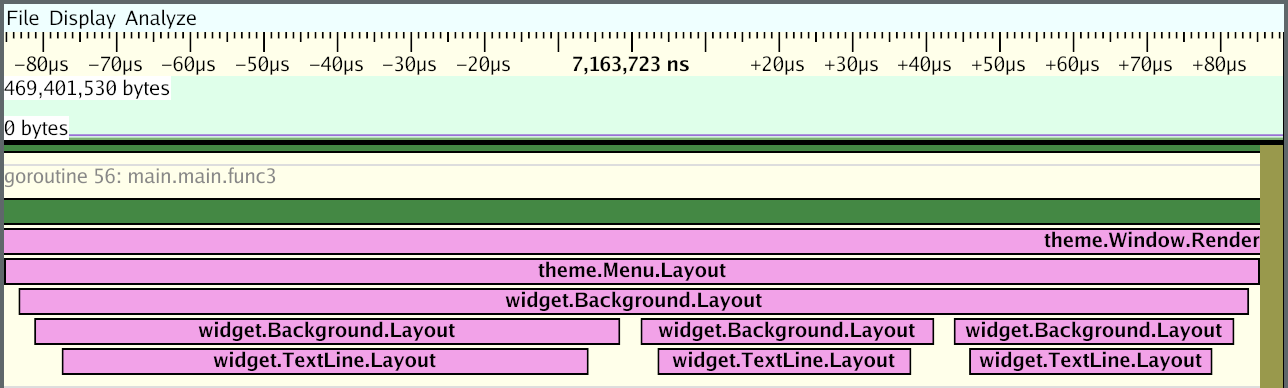
\includegraphics[width=\textwidth]{images/screenshots/user-regions.png}
  \caption{User regions showing how part of Gotraceui's \textsc{ui} is being rendered.}
\end{figure}

Finally, tasks exist to group work that is happening across multiple goroutines.
For example, if an incoming \textsc{api} request causes multiple goroutines to do work on behalf of that request in parallel, a task will be able to tie all of them together.
Tasks are created similarly to regions, but with \code{NewTask} and \code{(*Task).End} respectively.

Gotraceui does not currently display tasks.

\section{\code{net/http/pprof}}\label{net-http-pprof}

\code{net/http/pprof} is a package that adds \textsc{http} debugging endpoints to your application.
This is commonly used for acquiring \textsc{cpu} and memory profiles, but it can also be used to capture traces.
To collect a 5-second trace you can run a command like

\begin{verbatim}
curl -o trace.out http://localhost:6060/debug/pprof/trace?seconds=5
\end{verbatim}

There is no single endpoint to capture a trace with \textsc{cpu} profiling enabled, but you could capture both a \textsc{cpu} profile and a trace in parallel, like this:

\begin{verbatim}
curl -o /dev/null http://localhost:6060/debug/pprof/profile?seconds=6 &
curl -o trace.out http://localhost:6060/debug/pprof/trace?seconds=5
\end{verbatim}

We capture a slightly longer \textsc{cpu} profile to ensure it covers the entire duration of the trace.

\section{Tracing tests}

One way to acquire execution traces without having to modify your code is by using \code{go test}'s \code{-trace} flag, which writes an execution trace to a file.
This can be particularly useful in combination with running benchmarks.
You can additionally use the \code{-cpuprofile} flag to include \textsc{cpu} profiling samples in the trace.


\chapter{The user interface}
The following sections will describe the various components of Gotraceui's \textsc{ui}.

\section{Main window}
The main window displays a main menu and an interactive \noun{canvas} representing the trace data.
The canvas can be moved around by dragging with \keys{LMB}, by using the scroll wheel, or by using the scrollbar.
Holding \keys{\shortcut} while scrolling zooms in and out, centered around the cursor's position.
Dragging with \keys{\shortcut+LMB} selects a region of time to zoom to.
The \menu{Display} menu contains commands for changing the way \noun{timelines} are displayed on the canvas,
as well as commands for quick navigation.

\subsection{Axis}
The top of the window shows the \noun{axis}.
The bold tick indicates the origin of the axis and displays the absolute time at that point in the trace.
Ticks to the left and right of the origin show relative decrements and increments to this absolute time.

By default, the origin is placed at the center of the axis,
as analyzing traces often involves looking at what happened before and after an event.
The origin can be moved by clicking and dragging anywhere on the axis.
Alternatively, the context menu of the axis allows quickly placing the origin at the beginning, middle, or end of the axis.
Manually placed origins will stay in place when resizing the window or canvas,
while origins set via the context menu will stay at their relative position.

Additionally, the axis contains red and purple sections,
which correspond to the garbage collector's stop-the-world phase and general activity.
Pressing \keys{O} cycles through displaying the red section, both sections, or none of the sections across the entire canvas.

\subsection{Memory plot}

The axis is followed by the \noun{memory plot}, which shows memory usage (more specifically the size of the heap) and the garbage collector goal, using green and purple respectively.
Hovering anywhere on the plot will show a tooltip with the exact numeric values.
The memory plot is separated from the timelines by a black border.
This border can be clicked and dragged to resize the plot.

The plot's context menu offers the following additional features:

\begin{description}
\item[\menu{Hide/Show legends}] hides or shows the labels for the minimum and maximum value.
\item[\menu{Hide/Show \enquote{Heap size} series}] hides or shows the heap size.
\item[\menu{Hide/Show \enquote{Heap goal} series}] hides or shows the heap goal.
\item[\menu{Set extents to global extrema}] scales the plot so that the bottom represents the smallest measured value and the top represents the largest measured value, for the entire trace.
  Only the values of enabled series will be considered.
\item[\menu{Set extents to local extrema}] works like the previous command, but only considers the currently visible portion of the trace.
\item[\menu{Auto-set extents to local extrema}] automatically applies the previous command whenever the currently visible portion of the trace changes.
\item[\menu{Reset extents}] resets the extents to their default: zero at the bottom and the global maximum at the top.
\end{description}

\subsection{Timelines, tracks, and spans}
The main section of the canvas consists of a number of horizontally stacked timelines.
A timeline might show a processor, a goroutine, or phases of the garbage collector.
Every timeline has a label, hovering over which may display a tooltip.

For example, for processors, the tooltip will show how much time was spent executing user code,
doing garbage collection work,
and being idle.
Pressing \keys{\shortcut+LMB} on a label will zoom the canvas such that all spans in that timeline are visible.
Pressing \keys{LMB} on a goroutine label will open a panel with additional information about the goroutine (see \cref{panels} for more on panels.)

A timeline consists of one or more horizontally stacked \noun{tracks},
each track consisting of a series of \noun{spans}.
A span represents a state for some duration of time.
For example, a goroutine may be blocked on a channel send operation for \qty{100}{\milli\second}, and this would be displayed as a single span.
Tracks can visualize various things, such as the states of goroutines, call stacks, or user regions.

Hovering over a span will show context-specific information about it,
including its state and duration,
but also additional information such as tags (see \cref{tags})
or the reason for being in a certain state.
Pressing \keys{LMB} on a span will open a panel with additional information about the span, including a list of events that happened during that span.
Pressing \keys{\shortcut+LMB} on a span will zoom to the span.

Spans have different colors depending on the states they represent.
Different kinds of timelines and tracks use different color schemes.
These are explained in \cref{span-colors}.

Depending on the zoom level, individual spans may be too small to display.
Gotraceui uses two strategies to ensure that spans are always visible.
First, it merges consecutive tiny spans, displaying them as one big span instead.
Such merged spans get their own color.
Zooming into merged spans unmerges them.
Second, if there aren't enough spans to merge, the span is given a minimum size.

All spans have context menus, which include at least a \menu{Zoom} option, which acts identically to \keys{\shortcut+LMB}.
Some spans have more options:

\begin{itemize}
\item Spans in processor timelines have a \menu{Scroll to goroutine} option to scroll to the corresponding goroutine timeline.
\item Blocked spans in goroutine timelines have a \menu{Scroll to unblocking goroutine} option to scroll to the goroutine that unblocked the goroutine.
  For example, for a goroutine stuck in a channel receive, this will scroll to the sending goroutine.
\item Running spans in goroutine timelines have a \menu{Scroll to processor} option to scroll to the processor that the goroutine is running on at the time.
\end{itemize}

\subsubsection{Span colors}\label{span-colors}
Spans in processor timelines will have one of two colors:
\traceState{Green}{stateActive} for spans that represent running user goroutines,
and \traceState{purple}{stateGC} for spans that represent garbage collection work.

Spans in the first track of goroutine timelines can have many different colors,
representing the many different states a goroutine can be in.
You can find an exhaustive list of all goroutine states --- and the corresponding span colors --- in \cref{goroutine-states}.

User regions are displayed in \traceState{light pink}{stateUserRegion}.
Stack traces are displayed either in a \traceState{light shade of green}{stateStack} if they're from events,
or in a \traceState{lighter shade of green}{stateSampled} if they've been acquired via \textsc{cpu} sampling.

When small spans get merged, they will be displayed in one of two ways:
if all merged spans have the same state,
they will be displayed using a gradient from \traceState{light yellow}{stateMerged} to the color of the merged spans.
For merged spans with mixed states, a solid light yellow is shown instead.

\subsubsection{Span tags}\label{tags}
Gotraceui annotates spans with tags, which further describe the states goroutines are in.
These tags are produced by automatically parsing stack traces,
and for example deducing that a goroutine that's blocked on pollable \textsc{i/o} got to that state by making a \textsc{tls}-encrypted
\textsc{http} request over \textsc{tcp},
which provides a lot more information than just \enquote{\textsc{i/o}}.

Being based on stack trace parsing, tags are provided on a best-effort basis.
Without a matching, hand-written pattern, tags will not be recognized.
The authors add new patterns as they discover them and try to keep them in sync with new releases of Go.

The following tags exist:

\begin{itemize}
\item \code{\textsc{http}}, for \textsc{i/o} related to \textsc{http}
\item \code{\textsc{tcp}}, for \textsc{i/o} related to \textsc{tcp}
\item \code{\textsc{tls}}, for \textsc{i/o} related to \textsc{tls}
\item \code{accept}, for blocking on \href{https://man7.org/linux/man-pages/man2/accept.2.html}{accept(2)}ing\cite{AcceptLinuxManual2021} on a network connection
\item \code{dial}, for blocking on dialing a network connection
\item \code{network}, for network \textsc{i/o}
\item \code{read}, for read \textsc{i/o}
\end{itemize}

A single span can be annotated with multiple tags.


\subsubsection{Stack traces and \textsc{cpu} sampling}\label{cpu-sampling}
In addition to sequences of runtime events and user regions, Gotraceui can also display tracks for stack traces.
These can be enabled via \menu{Display>Show stack frames} or by pressing the \keys{S} key.
When using the keyboard shortcut, the timeline that is currently under the cursor will stay in its current position.
Other timelines will have to move, as their heights change due to the new tracks.

Each track represents one frame of the stack trace, with the frames sorted from bottom to top.
In other words, the first displayed frame represents the entry point of the goroutine.

There are two kinds of stack traces in Gotraceui: stacks associated with runtime events, and \textsc{cpu} sampling.
The first kind is straightforward to understand and conceptualize.
Most events that cause state transitions into blocked states, which cause new spans to be created, have stack traces associated with them.
These stacks are true for the entire duration of a span;
a span that is blocked on a channel receive in some function will be blocked at the same place the whole time, for example.

The second kind is trickier to understand. When \textsc{cpu} profiling is enabled during tracing, the trace will include \textsc{cpu} samples.
A \textsc{cpu} profiling sample states that at a specific point in time, a certain function was executing and how we got there.%
\footnote{More correctly, a sample states which instruction was executing and what the call stack looked like.
  In Gotraceui, we only consider the call stack.}
It doesn't say anything about what happened right before or after the sample.

By default, samples occur at a frequency of \qty{100}{\hertz}, i.e., once every \qty{10}{\milli\second}.
This means that there is \qty{10}{\milli\second} of uncertainty after a sample.
The stack trace might've changed anywhere from \num{0} to \qty{10}{\milli\second} after the sample.
The same function may even have been called repeatedly.
All we really know is that at one point in time, the function was running.

Displaying spans that are infinitely small, however, wouldn't be very useful.
For that reason, Gotraceui displays \textsc{cpu} samples similarly to how it displays stack traces of events.
A span for a \textsc{cpu} sample will start when the sample was made and it ends either when another sample is captured or when a state transition occurs.
To differentiate these less accurate stack traces from others, they are displayed in a lighter color.

The power of \textsc{cpu} samples lies in spotting macroscopic patterns in code execution, on the scales of hundreds of milliseconds, if not seconds.
A frame that gets sampled multiple times is likely to be spending more time executing than other frames.
To further aid this macroscopic view, spans of consecutive \textsc{cpu} samples that describe the same frame are merged.
This creates the usual layered representation of stacks that one might be familiar with from other tools such as flame graphs.

However, the data is woefully inadequate at small scales --- the kind of scales at which execution trace data exists.
You shouldn't rely on sampled stack traces to fill in the gaps between two runtime events that happened \qty{100}{\micro\second} apart.
It is important to either look at runtime events or \textsc{cpu} samples, but not both together.
Runtime events show an exact history of what happened in the runtime, while \textsc{cpu} samples show a guess at what happened in user code.

\begin{figure}[h]
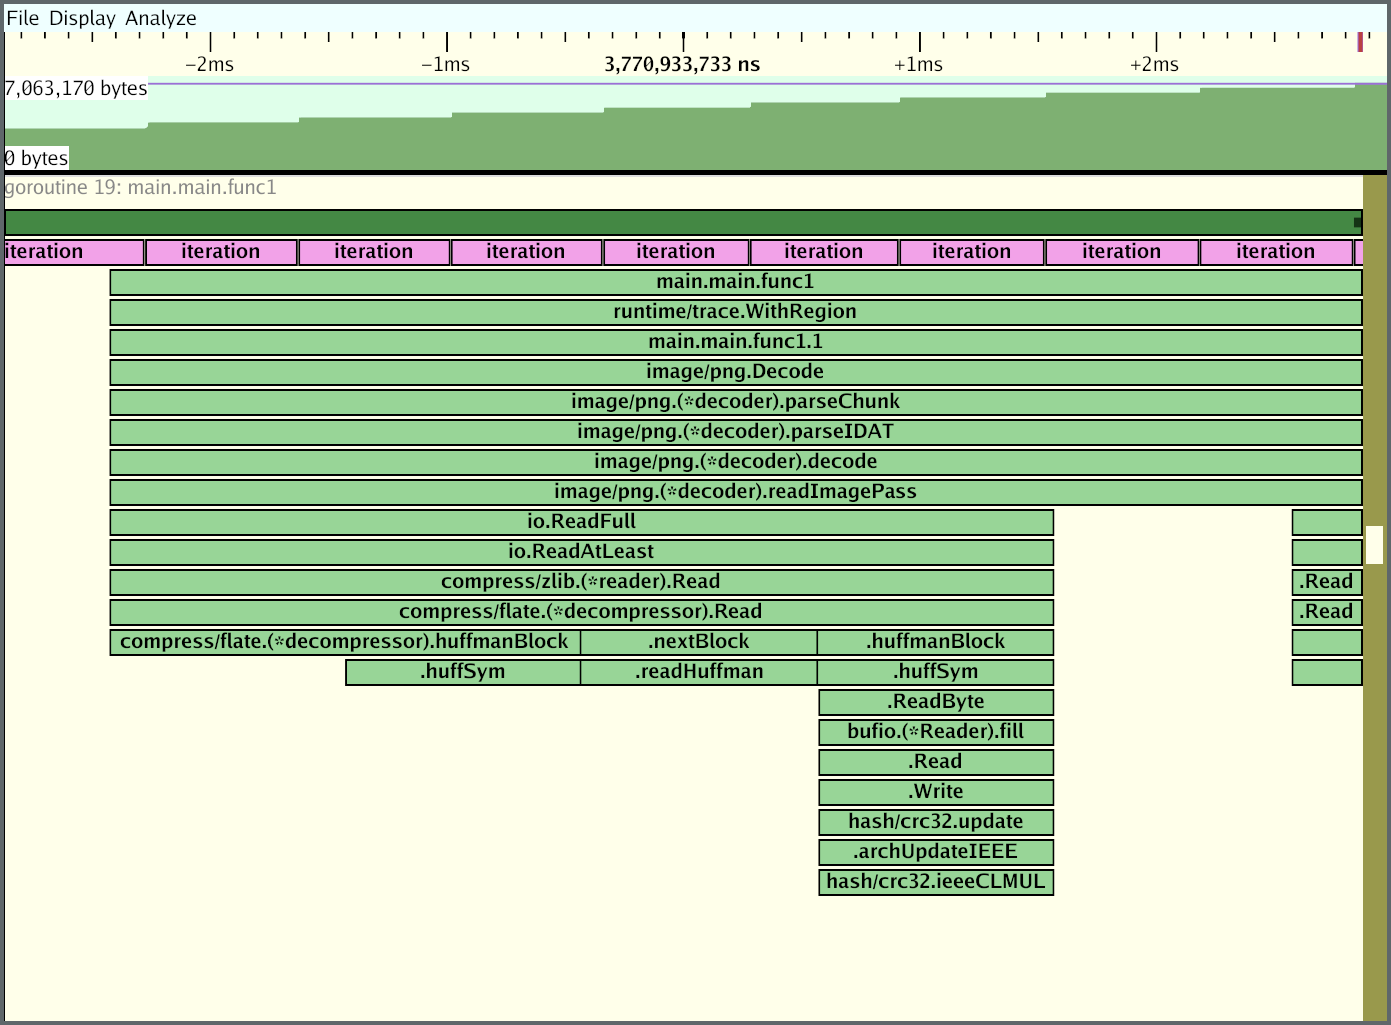
\includegraphics[width=\textwidth]{images/screenshots/sampling.png}
\caption{
  The trace of a loop parsing \textsc{png} files.
  Each pink span denotes an iteration.
  The \textsc{cpu} samples give us a rough idea of what was happening, but their resolution is quite coarse.
  There were six samples in total, which is less than one sample per iteration.
  We can be fairly certain that most time was spent somewhere in \code{readImagePass}, but beyond that we don't have enough data.
}
\end{figure}

It is also important to understand that \textsc{cpu} profiling samples happen at a fairly constant rate, which means all samples have the same uncertainty.
Runtime events, however, can happen at arbitrary points.
If a sample is followed by a runtime event \qty{1}{\milli\second} later then it will look much smaller than if it were followed by a runtime event \qty{9}{\milli\second} later,
even though in the latter case we still don't know what happened for the first \qty{9}{\milli\second}. 

\section{Links}

Timestamps and references to goroutines are formatted as clickable links.
Clicking on a timestamp will scroll the canvas to that point in time.
Clicking on a goroutine will display information about it in a goroutine panel.
Right-clicking on a goroutine opens a context menu that allows scrolling or zooming to the goroutine.

\section{Panels}\label{panels}

Gotraceui uses a side panel to display additional information about entities such as goroutines and spans.
Clicking on a supported entity opens the panel on the right side of the window.

Panels can be resized by dragging the black line, and they can be closed by pressing the \menu{Close} button in the top right.
Clicking \menu{Back} will go back to the previously displayed panel. This can be used repeatedly.
Finally, clicking \menu{Detach} will turn the panel into a standalone window.
Multiple panels can be detached at the same time.
A window can be turned back into a panel by clicking the \menu{Attach} button.

Depending on the type of panel, additional buttons may exist. 

\subsection{Goroutine panel}
\begin{itemize}
\item \todo{General information}
\item \todo{Stack trace}
\item \todo{Per-state statistics}
\item \todo{Events}
\end{itemize}

\subsection{Span panel}

\todo{TODO}

\section{Heatmaps}

Gotraceui can display processor utilization using quantized heatmaps.
These can be accessed via \menu{Analyze>Open processor utilization heatmap}.

The X-axis shows time, the Y-axis shows utilization in percent, and color saturation represents the number of processors.

The size of a bucket can be adjusted using the arrow keys. The \keys{\arrowkey{<}} and \keys{\arrowkey{>}} keys decrease and increase the amount of time represented by a bucket in steps of \qty{10}{\milli\second}.
The \keys{\arrowkey{v}} and \keys{\arrowkey{^}} keys decrease and increase the range of percentage points per bucket.

By default, a ranked color palette is used, where each distinct value that occurred gets its own saturation.%
\footnote{We are limited to 256 levels of saturation, but you probably don't have more than 256 processors in a utilization bucket.}
Compared to a linear palette, where the color is proportional to the value, a ranked palette makes it easier to spot outliers.
On the flip side, a linear palette allows comparing absolute values just by looking at the color.

\begin{figure}[h]
  \centering
  \begin{subfigure}[b]{0.49\textwidth}
    \centering
    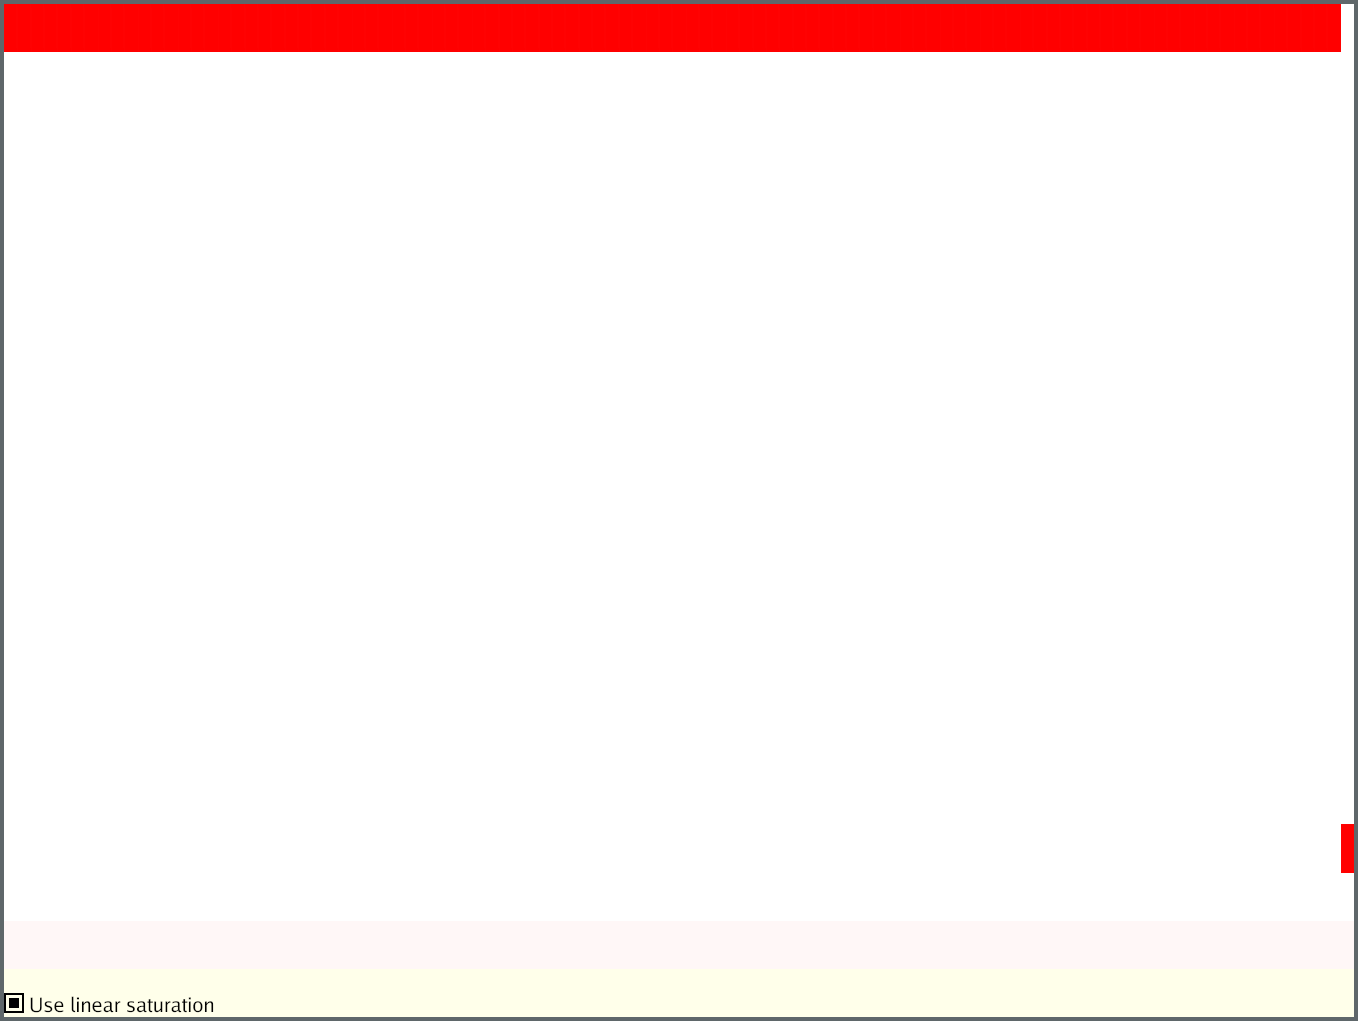
\includegraphics[width=\textwidth]{images/screenshots/heatmap-linear.png}
    \caption{Linear color palette.}
  \end{subfigure}
  \hfill
  \begin{subfigure}[b]{0.49\textwidth}
    \centering
    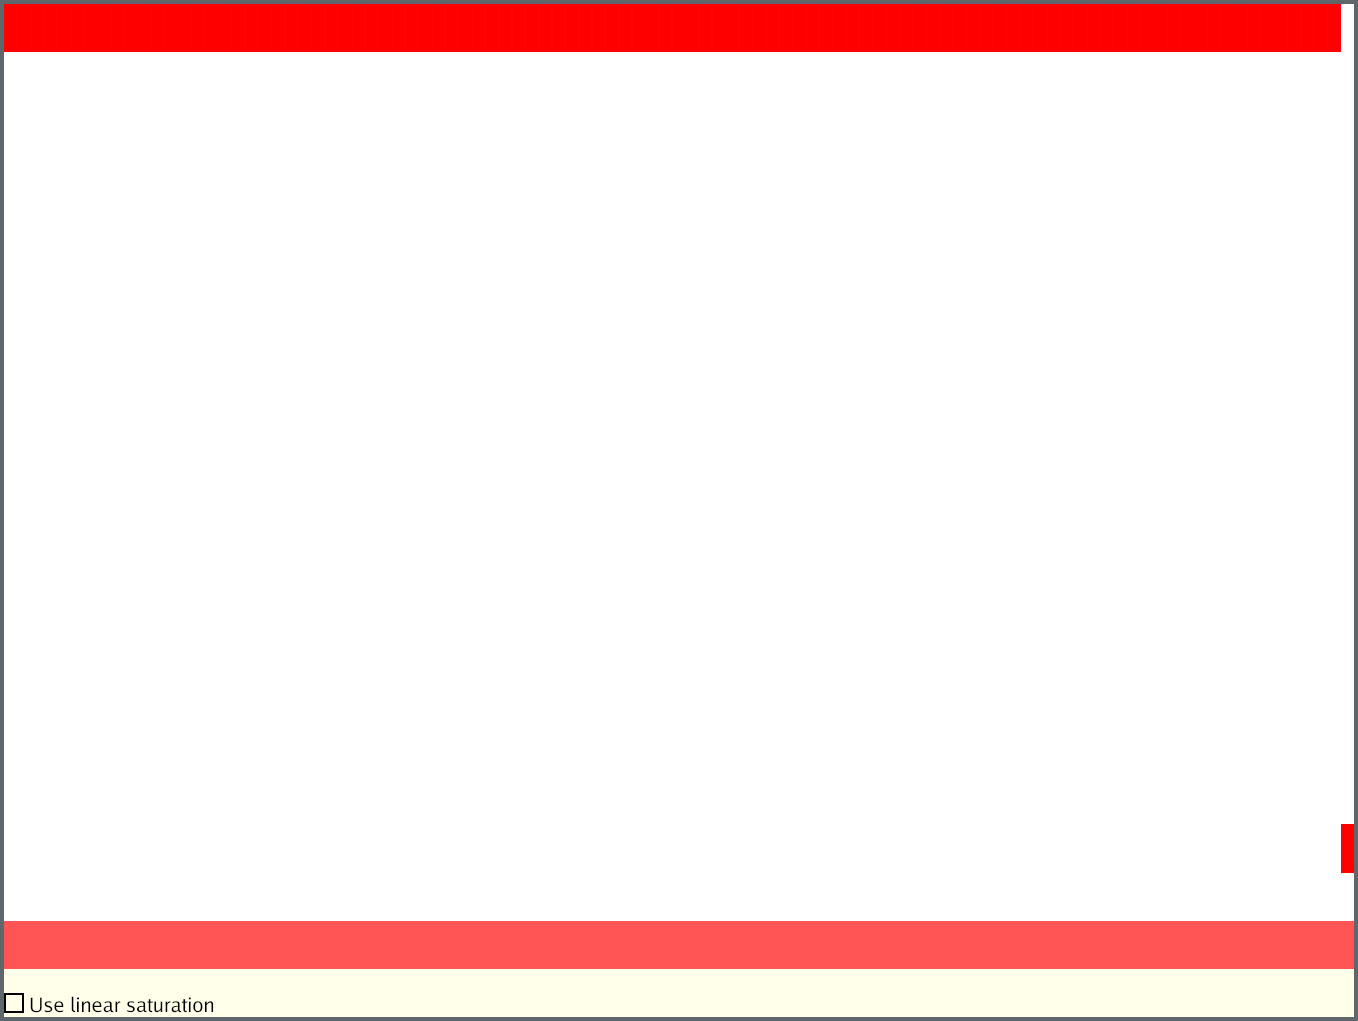
\includegraphics[width=\textwidth]{images/screenshots/heatmap-ranked.png}
    \caption{Ranked color palette.}
  \end{subfigure}

  \caption{Two heatmaps showing a trace with 31 processors at 95--100\% utilization and one processor at 0--5\% utilization. Note how on the left, the single processor is barely visible.}
\end{figure}

The bottom of the heatmap window displays information about the currently hovered bucket:
the range of time and the range of utilization represented by the bucket, as well as the number of processors in said bucket.

Please note that \emph{processor} refers to the concept from the Go runtime, and not actual \textsc{cpu}s or \textsc{cpu} cores.
While processor utilization is a good estimate for actual \textsc{cpu} utilization, it cannot account for the \textsc{os} scheduler, nor for cgo.



\section{Mouse and keyboard controls}

\subsection*{Main window}

\begingroup
\def\arraystretch{1.5}%
\begin{tabular}{ll}
  Input & Function \\
  \hline
  \keys{LMB} (click) & Open timeline and span information \\
  \keys{LMB} (drag) & Pan the canvas \\
  \keys{RMB} (click) & Open context menu \\
  \keys{\shortcut + LMB} (drag) & Zoom to selected area \\
  \keys{\shortcut + LMB} (click) & Zoom to clicked span or timeline \\
  % XXX scroll wheel
  % XXX shortcut + scroll wheel
  \keys{Home} & Scroll to top of canvas \\
  \keys{\shortcut + Home} & Zoom to fit currently visible timelines \\
  \keys{\shift + Home} & Jump to beginning of trace \\
  \keys{C} & Toggle compact display \\
  \keys{G} & Open timeline selector \\
  \keys{O} & Toggle \textsc{stw} and \textsc{gc} overlays \\
  \keys{S} & Toggle display of stack tracks \\
  \keys{T} & Toggle displaying tooltips \\
  \keys{X} & Toggle display of all timeline labels \\
  \keys{\shortcut + Z} &  Undo navigation
\end{tabular}
\endgroup

\subsection*{Heatmaps}

\begingroup
\def\arraystretch{1.5}%
\begin{tabular}{ll}
  Input & Function \\
  \hline
  \keys{\arrowkey{<}} & Decrease X-axis bucket size by \qty{10}{\milli\second} \\
  \keys{\arrowkey{>}} & Increase X-axis bucket size by \qty{10}{\milli\second} \\
  \keys{\arrowkey{v}} & Decrease Y-axis bucket size \\
  \keys{\arrowkey{^}} & Increase Y-axis bucket size
\end{tabular}
\endgroup


\chapter{The Go runtime}

Execution traces are primarily about the interactions between goroutines and the runtime.
To make sense of traces, then, it is helpful to understand how the runtime functions.
The following sections explain the most important aspects of the runtime and their impact on Gotraceui's visualization.

\section{The scheduler}
Go programs can have very many goroutines, up to millions.
Because it wouldn't be feasible to map one goroutine to one \textsc{os} level thread,
Go has to distribute goroutines over a smaller number of threads.
To do so, the scheduler has to decide which goroutines to run when,
part of which involves tracking which goroutines {\em can} run.
The activity related to this makes up a large part of what the trace captures and Gotraceui visualizes.
It is thus helpful to understand how the scheduler works.

\subsection{Machines, Processors, and Goroutines}

The scheduler manages three resources: \textbf{M}achines, \textbf{P}rocessors, and \textbf{G}oroutines.
In conversations, documentation, and source code these are usually referred to by their initials.

Machines correspond to operating system threads.
They are responsible for actually executing instructions.
Processors are, conceptually, tokens.
Machines need to hold processors to be allowed to run goroutines.
This serves two purposes:
First, it puts a bound on parallelism.
You wouldn't want hundreds of threads to fight for \textsc{cpu} resources.
Second, it allows for an efficient implementation.
While processors are tokens in principle, they are also a concrete data structure that holds information necessary for efficiently running goroutines.
In other words, machines use processors to run goroutines.
The environment variable \code{\textsc{gomaxprocs}} controls the number of available processors.
It defaults to the number of \textsc{cpu} cores.

In the context of execution traces and Gotraceui, goroutines are said to be running on processors, as the trace format is processor-centric.
In fact, Gotraceui does not expose machines at all.
If it did, it would show goroutines running on processors and processors running on machines.

If you'd like to learn more about the internals of the scheduler that aren't necessary to understand traces but are nevertheless interesting, check out \href{https://morsmachine.dk/go-scheduler}{Daniel Morsing's blog post on the topic}.\cite{morsingGoScheduler2013}

\subsection{Syscalls}\label{syscalls}
Syscalls, short for system calls, are the primary way that processes use to communicate with the operating system's kernel.
They are used to, for example, manipulate files, spawn new processes, use the network, etc.

Syscalls are synchronous: once a thread executes a syscall it cannot do anything else until the syscall returns.
When a goroutine executes a syscall it causes the whole machine to block --- that machine will not be able to run any other goroutines until the syscall returns.
When this happens, the machine loses its processor, after all it is no longer able to run goroutines, and another machine may pick up the processor.
Additionally, Go ensures that there are always enough unblocked machines to run all processors by creating new ones when necessary.

All of this work is fairly expensive.
That is why Go differentiates between ``non-blocking'' and ``blocking'' syscalls.
Non-blocking syscalls aren't truly non-blocking; they're just syscalls that return very quickly.
For example, the \code{gettimeofday} syscall usually returns within a few microseconds.
It would take longer to give up the processor and spawn a new thread than it would to wait for the syscall to return.
Additionally, the goroutine that invoked the syscall would have to wait its turn to be scheduled again, which might involve waiting for another goroutine to be preempted.
All in all, the cost of a cheap syscall would multiply tenfold.
Instead of doing all that, Go just waits to see if the syscall returns promptly\footnote{The exact duration it waits for depends on various factors, but it ranges from \num{0} to \qty{10}{\milli\second}.}.
Only if it doesn't will Go go through the steps we described earlier.

In the execution trace, and thus Gotraceui, these two kinds of syscalls are represented differently.
Short syscalls appear as instantaneous events during a span, while long syscalls appear as their own spans.

\subsection{\code{LockOSThread}}

By default, the scheduler moves goroutines between processors and processors between machines as necessary to maintain good performance.
For most Go programs, this is fine and indeed desirable.
However, when using cgo, it may be the case that the libraries you use depend on \emph{thread-local storage} (\textsc{tls}).
\textsc{Tls} allows storing per-thread state, which is little more than global variables scoped to threads.
Of course, if Go moves goroutines across threads, then thread-local state will not be available consistently.
To solve this problem, Go offers the \code{runtime.LockOSThread} function, which locks the current goroutine to the current thread.
From that point on, the goroutine will only ever run on that thread (unless \code{UnlockOSThread} is called), and no other goroutines will be allowed to run on it.

Because Gotraceui visualizes processors and goroutines but not machines, the use of \code{LockOSThread} is largely invisible.
In particular, thread-locked goroutines can still move between processors freely.

\subsection{Cooperative scheduling and preemption}

\todo{This section will be expanded in the future}

\subsection{Goroutine states}\label{goroutine-states}

All goroutines are in one of three states: Runnable, running, and blocked.
The runtime subdivides \emph{blocked} into different reasons for being blocked, and Gotraceui introduces some of its own subdivisions to further increase the level of detail.

The following is an exhaustive list of states found in Gotraceui.
Each state name's background color coresponds to the span color used in Gotraceui.

\begin{description}
\item[\traceState{created}{stateReady}:] Newly created goroutines will be in this state before they get scheduled for the first time.
  It is a special case of the ready state.

\item[\traceState{active}{stateActive}:] Active goroutines are those that are currently running.

\item[\traceState{send}{stateBlockedHappensBefore}, \traceState{recv}{stateBlockedHappensBefore},
  \traceState{select}{stateBlockedHappensBefore}:] These states describe the three ways in which goroutines can be
  blocked on channel communication.

\item[\traceState{sync}{stateBlockedHappensBefore}:] This state is used by goroutines that are blocked on sync
  primitives, such as \code{sync.Mutex}.

\item[\traceState{sync.Once}{stateBlockedHappensBefore}:] Blocked on a \code{sync.Once}.
  This is a special case of the sync state and detected by Gotraceui based on stack traces.

\item[\traceState{sync.Cond}{stateBlockedHappensBefore}:] Blocked on a condition variable (\code{sync.Cond}.)

\item[\traceState{I/O}{stateBlockedNet}:] This state is entered by goroutines that are waiting for pollable \textsc{i/o} to complete.
  See \cref{netpoller} for more information.

\item[\traceState{syscall}{stateBlockedSyscall}:] Goroutines enter this state when they invoke a blocking syscall.
  See \cref{syscalls} for an explanation of the difference between blocking and non-blocking syscalls in the context of Go.

\item[\traceState{blocked}{stateBlocked}:] Blocked goroutines are waiting for something to happen, but we don't know what.
  This usually happens for goroutines of the runtime that don't emit more accurate information.
  User goroutines will usually have more specific states such as \enquote{send}.

\item[\traceState{inactive}{stateInactive}:] This state is one of Gotraceui's custom states and is used for
  goroutines that are blocked or ready to run, but aren't actually eager to run.
  For blocked goroutines,
  this is exclusively used by goroutines of the runtime that block on some lock to pace the amount of work they do.
  Goroutines that are technically in the ready state but are marked inactive are those that called \code{runtime.Gosched} or \code{time.Sleep},
  as this indicates that they willingly gave up part of their share in \textsc{cpu} time,
  and their time spent waiting shouldn't be considered scheduler latency.

\item[\traceState{BlockedGC}{stateGC}:]  \todo{We still need to describe this state}

\item[\traceState{ready}{stateReady}:] A goroutine in this state isn't blocked on anything anymore and can start running
  as soon as it gets scheduled.
  A goroutine can be in this state because there aren't any free processors to run it,
  or simply because the scheduler hasn't gotten around to starting it yet.
  Goroutines can transition into this state from the active state if they get preempted,
  or from any of the various blocked states once they get unblocked.
  Time spent in this state is commonly called scheduler latency.

\item[\traceState{GC (idle)}{stateGC}:]  \todo{We still need to describe these states}

\item[\traceState{GC (dedicated)}{stateGC}:]  \todo{We still need to describe these states}

\item[\traceState{GC mark assist}{stateGC}:] Goroutines in the \enquote{\textsc{gc} mark assist} state are assisting the mark phase.
  See \cref{gc} to learn more about the garbage collector.

\item[\traceState{GC sweep}{stateGC}:] Goroutines in the \enquote{\textsc{gc} sweep} state are sweeping memory.
  See \cref{gc} to learn more about the garbage collector.

\item[stuck:] Goroutines in this state are stuck and can never make progress.
  This happens, for example, when receiving from a nil channel or using \code{select} with no cases.

\end{description}

\section{Pollable vs.\ non-pollable \textsc{i/o}}\label{netpoller}

To do \textsc{i/o} on files (we use \emph{files} in the Unix sense, referring to actual files, pipes, network connections, etc) we need to involve the operating system.
In \cref{syscalls} we established that this usually requires syscalls and indeed, the most straightforward way to read and write is to use the \code{read} and \code{write} syscalls (in the following we'll focus on reading, but everything applies equally to writing.)
However, we've also established that syscalls block execution and force Go to create new threads.
This is especially true for \textsc{i/o}, which rarely finishes quickly.
But what happens if we're working on a highly concurrent server that handles thousands of connections simultaneously?
We certainly do not want thousands of threads.
Threads are expensive to create, they need memory, the \textsc{os} has to manage them, the Go runtime has to manage them, and so on.
Avoiding a large number of threads is one of the reasons Go doesn't use one thread per goroutine in the first place.

Most operating systems provide a more efficient alternative to having thousands of threads waiting in syscalls:
a combination of non-blocking \textsc{i/o} and some mechanism that can be polled to wait for files to become ready.
Non-blocking means that instead of blocking, read syscalls fail immediately if there is no data available to be read.
The expectation is that the program will try again in the future.
Ideally this is combined with the aforementioned polling-based mechanism which tells the program when a file is ready to be read from.
Using these two features means that we no longer need one thread per outstanding \textsc{i/o} operation. Instead, we need one thread to poll for events, and some number of threads to do \textsc{i/o}.

In a low-level language like C, we'd be responsible for managing non-blocking \textsc{i/o}, polling, retrying reads, and possibly using a thread pool.
In Go, all of this is hidden from view. To the programmer, all reads look like ordinary blocking calls: \code{f.Read(b)} will return once it has read some data.
In the background, however, the runtime uses the features we've described previously.
A read doesn't map to a simple syscall. Instead, it calls into the runtime, which is responsible for reading, polling, and retrying.
During polling, the goroutine is put into a blocked state and the processor that was running it is free to run other goroutines.
Once the file becomes ready for reading, the goroutine is unblocked and scheduled so it can retry the read.

The runtime system responsible for polling is called the \emph{netpoller}. It is called that because originally, it only supported network connections.
Since then it has been expanded to operate on other kinds of files, too, such as pipes.
However, not all kinds of files are pollable. For example, Go uses epoll on Linux, and epoll doesn't support ordinary disk files.
Which kinds of files are pollable also differs between operating systems, as each \textsc{os} provides its own mechanism.
For non-pollable files the netpoller cannot be used and Go falls back to normal, blocking syscalls, with all of the previously mentioned downsides.
However, the most important use case of the netpoller is undoubtedly network connections, and these are pollable on all systems.

In Gotraceui, blocking on pollable \textsc{i/o} is represented using \textsc{i/o} spans, while non-pollable \textsc{i/o} is shown as syscalls in the way described in \cref{syscalls}.
For pollable \textsc{i/o}, span tooltips may additionaly show the kind of \textsc{i/o}, such as network reads. This information is based on tags, which are described in \cref{tags}.

\begin{figure}[h]
  \centering
  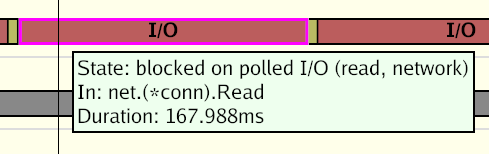
\includegraphics[scale=2]{images/screenshots/pollable-io-span.png}
  \caption{A span blocked on a pollable network read.}
\end{figure}

\section{Garbage collection}\label{gc}
Go uses a concurrent mark and sweep garbage collector.
Its activity will interact with the scheduling of your goroutines in various ways,
which we'll explore in this section.
We will focus on the details that matter for understanding execution traces.
There are many more details to how the \textsc{gc} works
and you're encouraged to read the \href{https://go.dev/doc/gc-guide}{official documentation}\cite{GuideGoGarbage} to learn more about it.

% \todo{Something about mark, sweep, mark assist, STW, how GC gets triggered, etc}

\todo{This section will be expanded in the future}

\section{The runtime's goroutines}
The runtime spawns several of its own goroutines that will show up in most traces.
Most of these exist to help with the concurrent garbage collector.

\begin{itemize}
\item \code{bgsweep} is a low priority goroutine that sweeps spans when there are idle processors. This reduces the amount
  of sweeping that has to be done by other goroutines.
\item \todo{bgscavenger}
\item \todo{gcBgMarkWorker}
\item \code{forcegchelper} periodically gets woken up and forces a garbage collection cycle to start.
  This ensures that garbage gets collected regularly even if the program isn't allocating enough memory to hit the heap target.
\item \code{runfinq} is the goroutine that is responsible for running finalizers.
  That means that this runtime goroutine will execute code provided by the user via \code{runtime.SetFinalizer}.
\end{itemize}

\chapter{Final words}

The best way to get started with runtime tracing is to jump right in.
\enlargethispage{3\baselineskip}
\begin{figure}[h!]
  \centering
  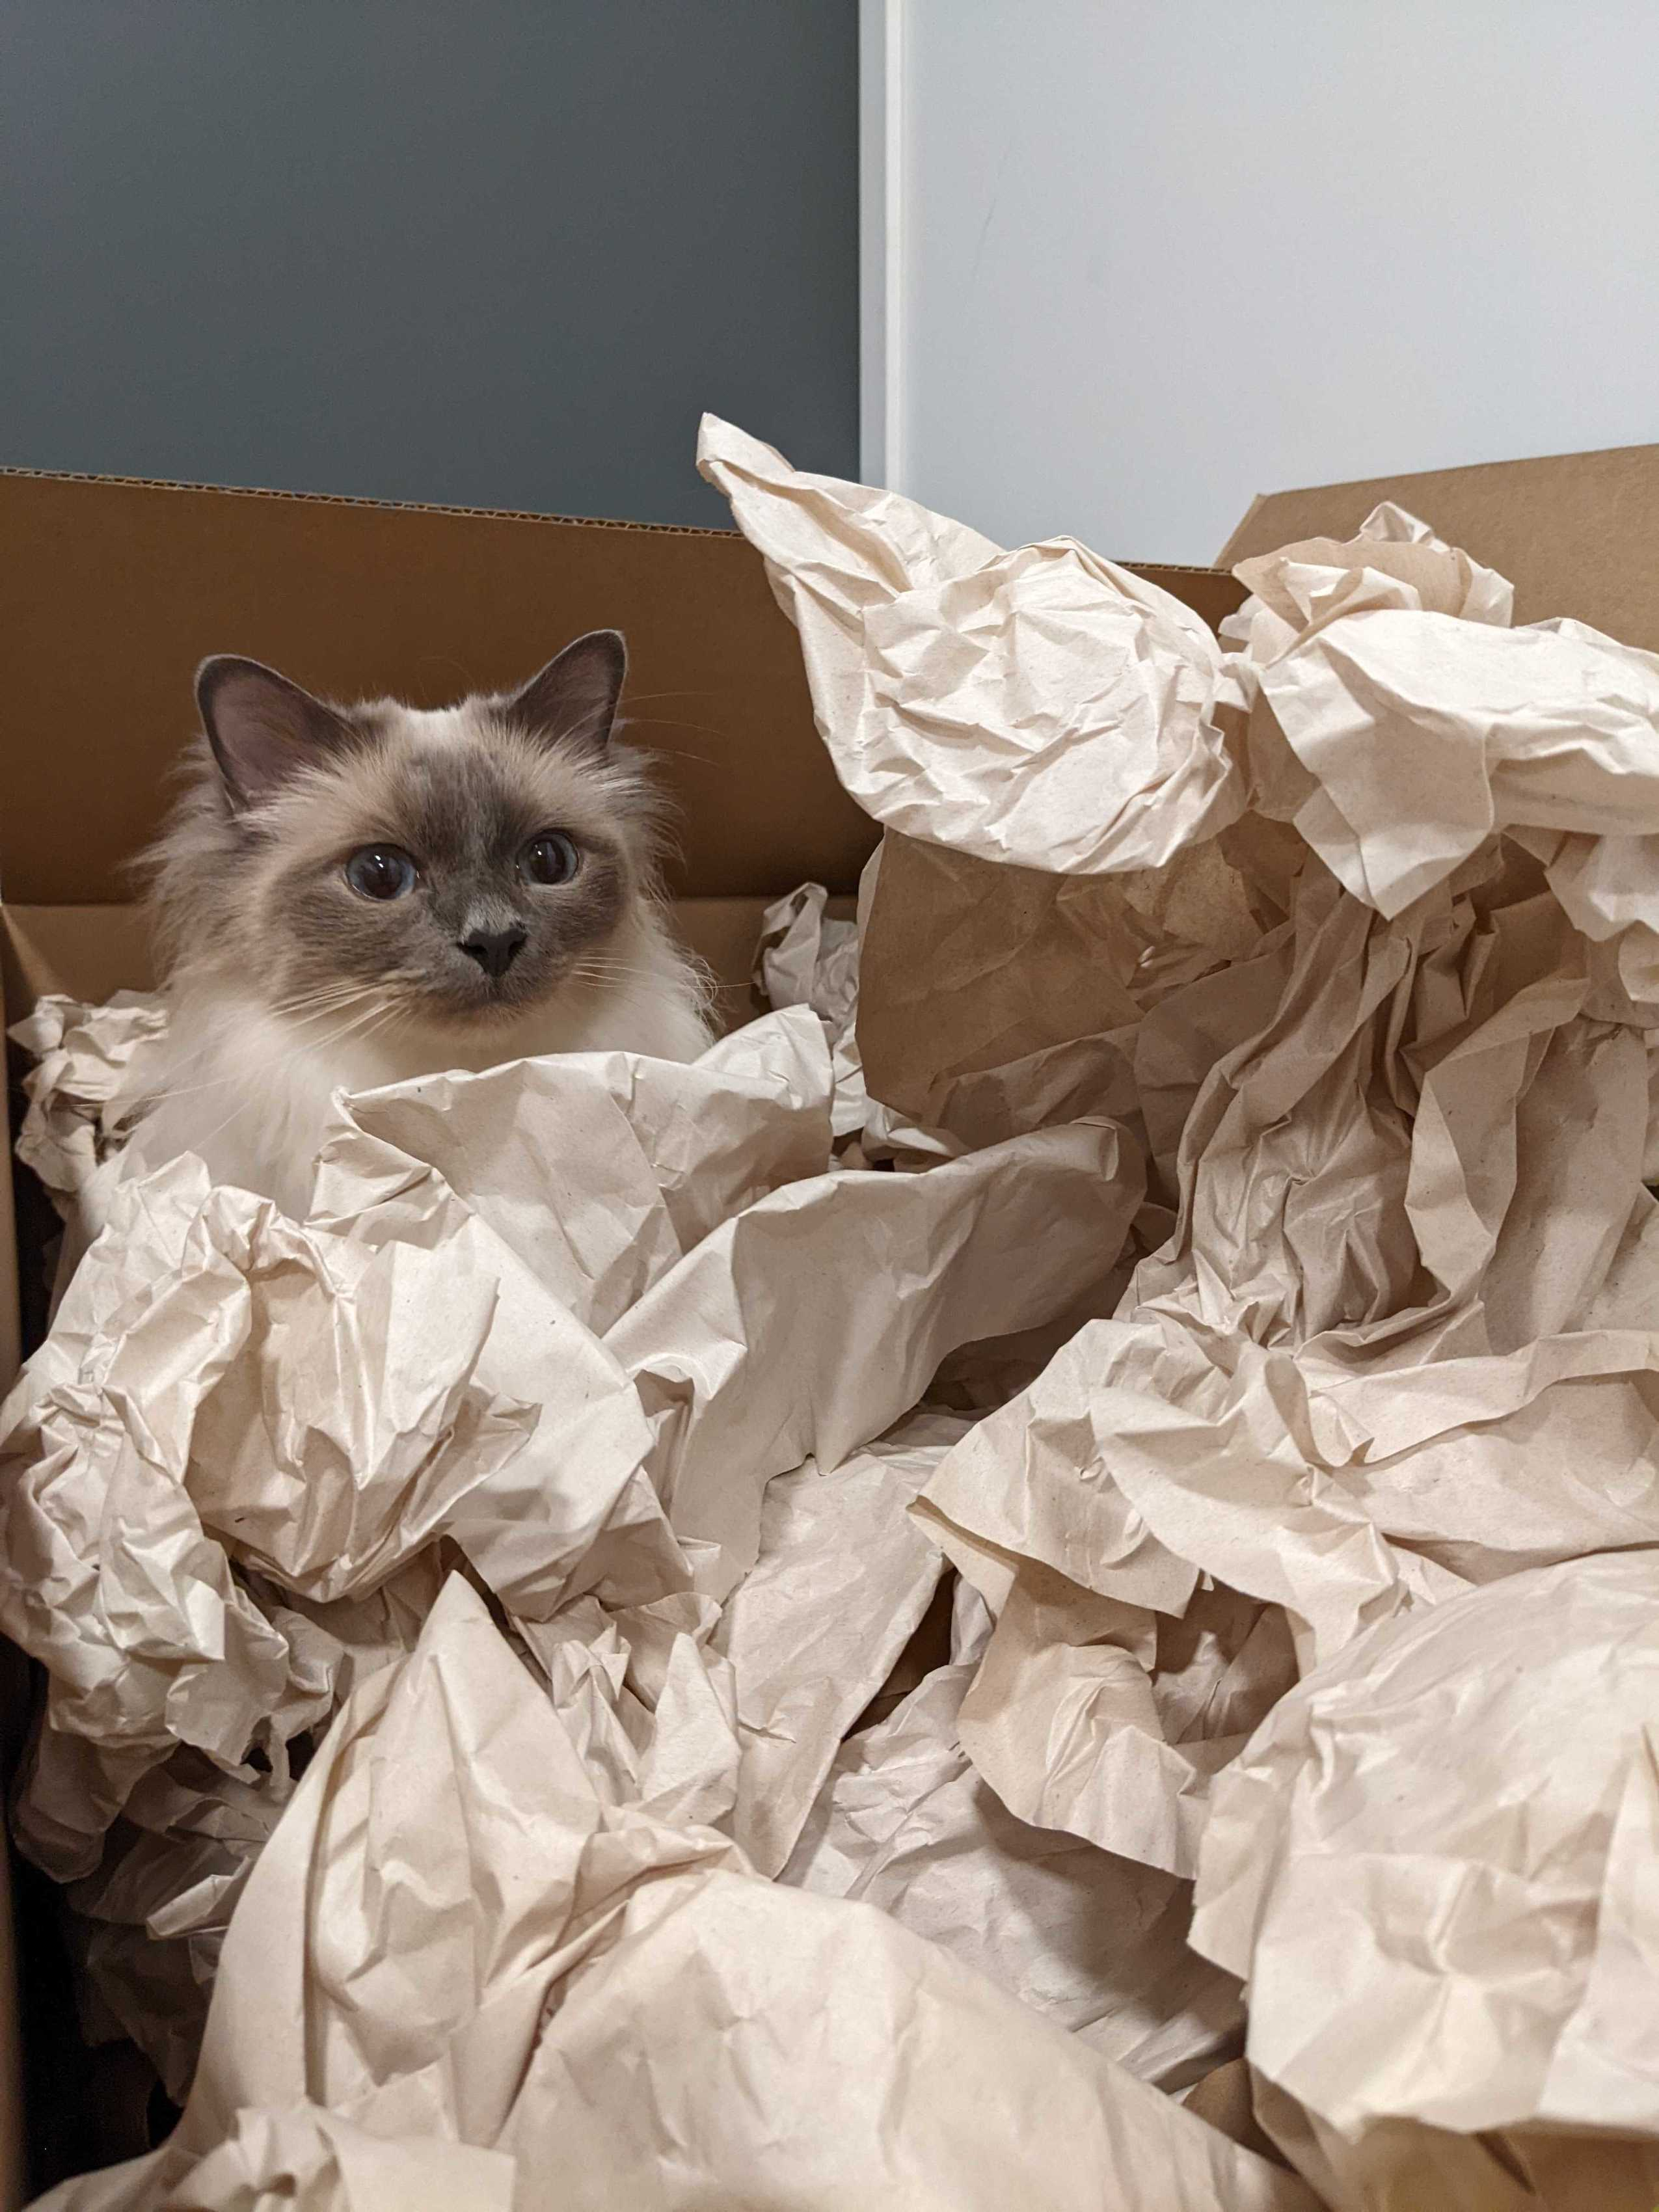
\includegraphics[width=0.6\textheight]{images/olive.jpg}
  \caption*{Olive, who is the bestest.\\\textcopyright{}~\href{https://catzkorn.dev/}{Charlotte Brandhorst-Satzkorn}, Olive's owner.}
\end{figure}


\backmatter

\printbibliography

\end{document}
